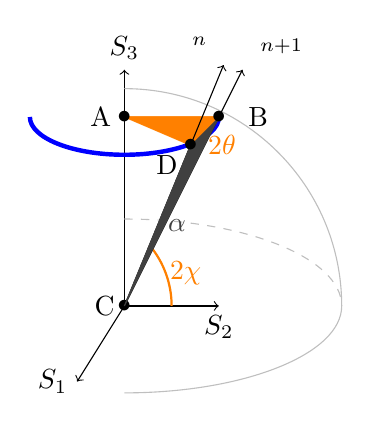
\begin{tikzpicture}[scale = 1.2]
    \node (C) at (0,0) {$\bullet$} node[left]{C};
    \node (A) at (0,2) {};
    \node (B) at (1,2) {};
    \node (D) at (0.7,1.7) {$\bullet$};
    \draw[->] (C.center) --++ (0,2.5) node[above]{$S_3$};
    \draw[->] (C.center) --++ (1,0) node[below]{$S_2$};
    \draw[->] (C.center) --++ (-0.5,-0.8) node[left]{$S_1$};

    \draw[lightgray, thin] (0,2.3) arc (90:0:2.3);
    \draw[lightgray, thin] (0,-0.92) arc (90:0:2.3cm and -0.92cm);
    \draw[lightgray, thin, dashed] (0,0.92) arc (90:0:2.3cm and 0.92cm);


    \draw[ultra thick, blue] (1,2) arc (180:0:-1cm and -0.4cm);
    \draw[thick, orange] (0.5,0) arc (0:40:1cm) node[midway, xshift = 0.25cm]{$\bm{2\chi}$};
    \filldraw[color= orange] (A.center) -- (B.center) to[bend left = 20] (D.center)node[right = 0.1cm, orange]{$\bm{2\theta}$};
    \filldraw[orange, opacity = 0.85] (A.center) -- (B.center) to[bend left = 20] (D.center) -- (A.center);
    
    \draw[->] (C.center) --++ (1.25,2.5) node[xshift = 0.5cm, yshift = 0.3cm]{$\vecS_{n+1}$};
    \draw[->] (C.center) --++ (1.05,2.55) node[xshift = -0.3cm, yshift = 0.3cm]{$\vecS_{n}$};

    \filldraw[color= gray!50!black] (B.center) -- (C.center) -- (D.center)node[midway, xshift = 0.25cm]{$\bm{\alpha}$};
    
    \draw (A) node{$\bullet$} node[left of=A, xshift = 0.7cm] {A};
    \draw (B) node{$\bullet$} node[right of=B, xshift = -0.5cm] {B};
    \draw (D) node{$\bullet$} node[left of=D, xshift = 0.7cm, yshift = -0.25cm] {D};
\end{tikzpicture}
